
\documentclass{llncs}
\usepackage{graphicx}
\usepackage{lipsum}
\usepackage{float}
\usepackage{url}
\usepackage{listings}
\usepackage{xcolor}
\usepackage{amsmath}
\usepackage{amssymb}

\lstset{
    basicstyle=\ttfamily\small,
    keywordstyle=\color{blue},
    commentstyle=\color{gray},
    stringstyle=\color{red},
    breaklines=true,
    frame=single
}

\begin{document}
%
\title{Deepfusion Language Model}

\author{Nguyen Trong Minh - 2540074\and
Nguyen Duc Duy - 2540043 \and Bui Dang Quang - 2540092}

\institute{University of Science and Technology of Hanoi, Vietnam\\}
\maketitle

\begin{abstract}
We built a masked diffusion language model for Vietnamese from scratch, following
the recipe in LLaDA. The model has about 73 million parameters and uses bidirectional
attention instead of the usual left-to-right causal mask. We trained our own byte-pair
tokenizer, pretrained on a corpus of 10{,}000 Vietnamese books, continued pretraining on
a Vietnamese history question-answering set, and then fine-tuned on the diffusion objective
described in the LLaDA paper. On a held-out test set of 1{,}000 examples we measured a
corpus perplexity of 104.7 with the low-variance likelihood estimator from the paper. That is
far below the random baseline of 8{,}192 (our vocabulary size) but still well short of a strong
model, which tells us the model learned real structure in the language while remaining limited
by its size and the amount of data we could train on.

\keywords{diffusion language models \and masked language modeling \and Vietnamese NLP}
\end{abstract}

\section{Introduction}

Most language models today predict one token at a time, left to right. LLaDA \cite{llada}
asks a different question: do we actually need the autoregressive part, or is it the
generative training objective that matters? It answers by training a diffusion model that
masks tokens at random and learns to fill them back in. There is no causal mask, so the
model sees the whole sequence at once and can attend in both directions.

We wanted to reproduce that idea on a smaller scale and in a language we care about. This
report describes Deepfusion, our Vietnamese masked diffusion model. We did everything from
the ground up: the tokenizer, the architecture, the pretraining, and the fine-tuning. The
goal was not to beat a large model. It was to get the full pipeline working end to end and
to see how far a 73M-parameter diffusion model can go on a modest Vietnamese corpus.

The training has two ideas worth stating up front. During pretraining we mask tokens across
the whole text and ask the model to recover them, which is masked language modeling with a
random mask ratio rather than the fixed 15\% that BERT uses. During fine-tuning we keep the
prompt intact and only mask the answer, so the model learns the conditional distribution of a
response given a question. Both stages share the same loss; the difference is which tokens get
masked.

\section{Model architecture}

Our model, \texttt{DeepfusionLM}, borrows from the ModernBERT design. It is a stack of twelve
Transformer blocks with a hidden size of 768 and twelve attention heads. The full count comes
to 73{,}382{,}912 trainable parameters. Each block has a pre-norm attention layer and a
gated feed-forward layer, both wrapped in residual connections.

A few design choices are worth calling out.

\textbf{Bidirectional attention.} Because the model predicts masked tokens, it has no reason
to hide future positions. Every token attends to every other token. We implement this with
PyTorch scaled dot-product attention and a mask convention where a value of one means ``attend
to this position'' and zero means padding.

\textbf{Rotary position embeddings.} We use RoPE \cite{rope} on the queries and keys inside
each head rather than learned absolute positions.

\textbf{Mixed attention windows.} Most layers use a sliding window of 128 tokens so that
attention stays local and cheap. Every third layer switches to full attention over the whole
sequence and uses a larger RoPE base of 160{,}000 so it can carry longer-range information.
The idea is that local layers handle nearby context and the occasional global layer ties the
sequence together. (We later experimented with dropping the sliding window in favor of full
attention everywhere; the architecture supports both.)

\textbf{Gated feed-forward.} The feed-forward block uses a GeGLU gate: it projects up, splits
the result in two, passes one half through GELU, and multiplies the halves together before
projecting back down.

The output head is a small decoder: a dense layer, a GELU, a layer norm, and a final
projection to the 8{,}192-token vocabulary.

\section{Tokenizer}

We trained a byte-pair encoding tokenizer with a vocabulary of 8{,}192 on the same Vietnamese
book corpus we used for pretraining. Before training we normalized every line to Unicode NFC
form and stripped characters outside the Vietnamese alphabet, digits, and basic punctuation.
NFC matters for Vietnamese because the same accented letter can be encoded in more than one way,
and we did not want the tokenizer to waste vocabulary on duplicates.

The tokenizer reserves seven special tokens: \texttt{[UNK]}, \texttt{[START\_ID]},
\texttt{[END\_ID]}, \texttt{[EOT]}, \texttt{[MASK]}, \texttt{[BOS]}, and \texttt{[EOS]}. We
reuse \texttt{[EOS]} as the padding token. The \texttt{[START\_ID]} and \texttt{[END\_ID]}
tokens wrap role names in the chat template so the model can tell where a user turn ends and an
assistant turn begins.

\section{Pretraining}

We pretrained on a dataset of 10{,}000 Vietnamese books from Kaggle. The text is tokenized and
packed into fixed chunks of 1{,}024 tokens, with an \texttt{[EOS]} token between documents.

The training objective is the LLaDA forward process. For each sequence we draw a masking ratio
$t$ uniformly from $(0, 1)$, then mask each token independently with probability $t$. The model
sees the corrupted sequence and predicts the original tokens at the masked positions. We compute
cross-entropy only on those positions and scale each sample's loss by $1/t$:

\begin{equation}
\mathcal{L}(\theta) = -\,\mathbb{E}_{t,\,x_0,\,x_t}
\left[ \frac{1}{t} \sum_{i=1}^{L} \mathbf{1}\!\left[x_t^i = \mathbf{M}\right]
\log p_\theta\!\left(x_0^i \mid x_t\right) \right].
\end{equation}

The $1/t$ term keeps the objective fair. When $t$ is large most of the sequence is masked, which
is a much harder problem, so without rescaling those samples would dominate the loss. We are also
careful never to mask padding tokens.

We trained with the AdamW optimizer, a cosine learning-rate schedule with warmup, mixed-precision
(fp16), and gradient accumulation, all managed through HuggingFace Accelerate. Checkpoints are
written periodically so we can resume.

\section{Continued pretraining}

A book corpus teaches general Vietnamese but says little about the kind of factual,
question-shaped text we cared about. So we ran a second pretraining stage on the
Vietnam-History-200K question-answering dataset. The objective is identical to the first stage:
random-ratio masking over the whole sequence. The only changes are a smaller learning rate and a
shorter schedule, since we are adapting an already-trained model rather than starting over. This
step nudges the model toward the vocabulary, names, and phrasing of Vietnamese history before we
ask it to follow instructions.

\section{Supervised fine-tuning}

The last stage is where the diffusion objective from LLaDA does its real work. We format each
example with a chat template that marks the user question and the assistant answer, then build a
mask that marks which tokens belong to the answer. During training we leave the question alone and
only mask answer tokens:

\begin{equation}
-\,\mathbb{E}_{t,\,p_0,\,r_0,\,r_t}
\left[ \frac{1}{t} \sum_{i=1}^{L'} \mathbf{1}\!\left[r_t^i = \mathbf{M}\right]
\log p_\theta\!\left(r_0^i \mid p_0,\, r_t\right) \right].
\end{equation}

Here $p_0$ is the prompt, $r_0$ is the answer, and $r_t$ is the answer with tokens masked at ratio
$t$. The model learns $p_\theta(r_0 \mid p_0)$, the distribution of an answer given a question. We
also divide each sample's loss by its answer length so that long answers do not count more than
short ones.

At inference time generation runs the reverse process. We start with a fully masked answer and
unmask it over a number of steps, predicting all masked positions at once and then remasking some
of them for the next step. We support two remasking strategies: plain random remasking, and the
low-confidence strategy from the paper that keeps the most certain predictions and re-masks the
rest. By default we decode greedily.

\section{Results}

\subsection{Training convergence}

Figure~\ref{fig:loss} shows the training and validation loss over the fine-tuning run. The
training loss starts near 0.29 and falls quickly, settling around 0.045 by the tenth epoch. The
validation loss starts lower, drops to about 0.07, and then flattens out. The two curves cross
near epoch four or five. After that the training loss keeps dropping while the validation loss
holds steady and even ticks up a little, which is the usual sign of mild overfitting. In practice
the best checkpoint to keep is the one near that crossing point, before the gap opens up.

\begin{figure}[H]
\centering
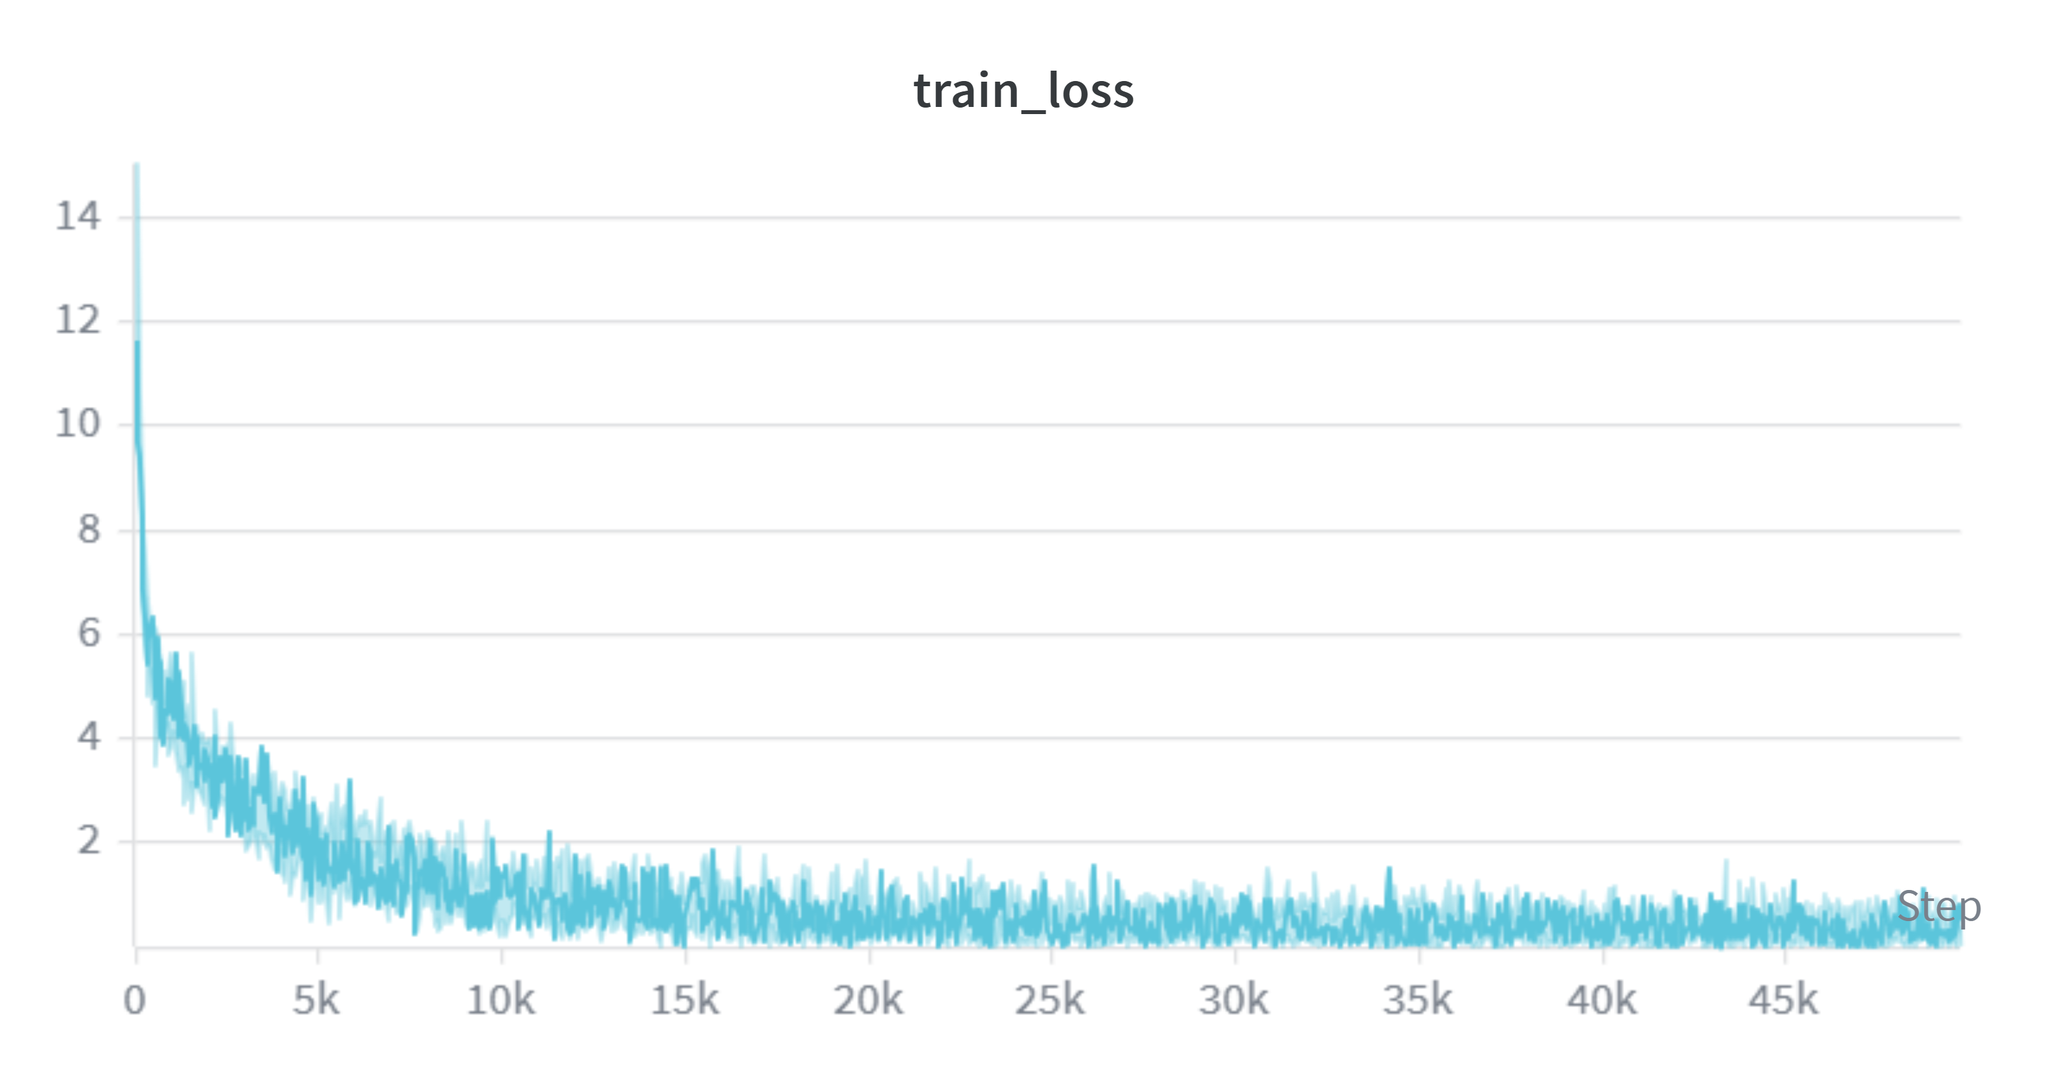
\includegraphics[width=0.8\textwidth]{images/training-loss-graph.png}
\caption{Training and validation loss during supervised fine-tuning. The validation loss bottoms
out around epoch five, after which the model begins to overfit.}
\label{fig:loss}
\end{figure}

\subsection{Likelihood evaluation}

Training loss is convenient but noisy, because each batch uses a single random masking ratio. To
get a more stable number we used the lower-variance estimator from the paper, which masks exactly
$l$ response tokens chosen at random and averages over many draws:

\begin{equation}
-\,\mathbb{E}_{l,\,r_0,\,r_l}
\left[ \frac{L}{l} \sum_{i=1}^{L} \mathbf{1}\!\left[r_l^i = \mathbf{M}\right]
\log p_\theta\!\left(r_0^i \mid p_0,\, r_l\right) \right].
\end{equation}

We evaluated on 1{,}000 held-out examples, 50{,}207 response tokens in total, with 128 Monte Carlo
draws per example. Table~\ref{tab:results} reports the numbers.

\begin{table}[H]
\centering
\caption{Conditional likelihood on the held-out test set (1{,}000 examples, 128 Monte Carlo draws
per example).}
\label{tab:results}
\begin{tabular}{lr}
\hline
Metric & Value \\
\hline
Mean per-example log-likelihood (higher is better) & $-233.53$ \\
Mean per-token negative log-likelihood (lower is better) & $4.65$ \\
Corpus perplexity (lower is better) & $104.73$ \\
\hline
\end{tabular}
\end{table}

A perplexity of 104.7 means that, on average, the model is about as unsure as if it were choosing
among 105 tokens at each step. Our vocabulary has 8{,}192 tokens, so a model that learned nothing
would sit near that number. Coming down to 105 shows the model captured a lot of real structure.
At the same time, a strong model lands in the single digits, so we are still a long way from that.
We read this as an honest middle result: the pipeline works and the model learned Vietnamese, but
73M parameters and our data budget put a ceiling on how good it can get.

\section{Discussion and limitations}

The clearest limit is scale. LLaDA was trained on trillions of tokens at 8 billion parameters.
We trained a model two orders of magnitude smaller on a corpus many orders smaller than that, so
the gap in perplexity is expected. The overfitting we saw during fine-tuning also points at the
size of the instruction data: with more question-answer pairs the validation curve would likely
keep falling for longer.

There are some rough edges in the code we would tidy up given more time. The masking convention in
one of the older inference scripts is inverted relative to the rest of the project, and several
paths are hard-coded to the machine we trained on. Neither affects the results, but both would trip
up someone trying to rerun the work.

What did work well was the diffusion setup itself. Bidirectional attention and the random-ratio
masking objective trained without trouble, and the reverse-process sampler produces readable
Vietnamese for short prompts. For a first attempt at a non-autoregressive model, that is the part
we are happiest with.

\section{How to run the project}

The pipeline runs in stages. Each stage produces an artifact that the next stage consumes, so the
order matters. The commands below assume you are in the project root.

\medskip
\noindent\textbf{1. Install dependencies.}
\begin{lstlisting}[language=bash]
pip install -r requirements.txt
\end{lstlisting}

\noindent\textbf{2. Configure paths.} Create a \texttt{.env} file in the project root pointing at
your data and tokenizer locations:
\begin{lstlisting}[language=bash]
CORPUS_PATH=/path/to/vietnamese-books
TOKENIZER_PATH=./DeepfusionLM_tokenizer
PROCESSED_PRETRAIN_DATA_PATH=./tokenized_vietnamese_book
\end{lstlisting}

\noindent\textbf{3. Train the tokenizer} on the book corpus.
\begin{lstlisting}[language=bash]
python train_tokenizer.py
\end{lstlisting}

\noindent\textbf{4. Attach the chat template} and save the tokenizer directory used by every
later stage.
\begin{lstlisting}[language=bash]
python prepare_chat_template.py
\end{lstlisting}

\noindent\textbf{5. Tokenize the pretraining corpus} into fixed 1{,}024-token chunks.
\begin{lstlisting}[language=bash]
python tokenize_pretrain_data.py
\end{lstlisting}

\noindent\textbf{6. Pretrain} the model with the masked diffusion objective. We launch through
Accelerate so the run can use mixed precision and multiple GPUs.
\begin{lstlisting}[language=bash]
accelerate launch pretrain.py
\end{lstlisting}

\noindent\textbf{7. Download the history QA dataset} for the second pretraining stage.
\begin{lstlisting}[language=bash]
python download_dataset.py
\end{lstlisting}

\noindent\textbf{8. Continue pretraining} on the QA data. This script takes command-line
arguments for the checkpoint path, learning rate, and schedule.
\begin{lstlisting}[language=bash]
python continued-pretrain.py --model_weight_dir my_experiment/checkpoint_120000
\end{lstlisting}

\noindent\textbf{9. Prepare the supervised fine-tuning data.} This applies the chat template and
builds the answer mask.
\begin{lstlisting}[language=bash]
bash run_prepare_sft_data.sh
\end{lstlisting}

\noindent\textbf{10. Fine-tune} on the diffusion objective. Edit the GPU id and paths at the top
of the script first, then run it.
\begin{lstlisting}[language=bash]
bash run_finetune_sft.sh
\end{lstlisting}

\noindent\textbf{11. Generate} from a fine-tuned checkpoint. Omit \texttt{--prompt} for
unconditional generation.
\begin{lstlisting}[language=bash]
python inference_sft.py --prompt "<your Vietnamese question here>" \
    --strategy low_confidence --num_steps 512
\end{lstlisting}

\noindent\textbf{12. Evaluate} the likelihood on the held-out test set.
\begin{lstlisting}[language=bash]
python evaluate_likelihood.py --n_mc 128
\end{lstlisting}

\medskip
\noindent To watch training while it runs, start TensorBoard with
\texttt{bash start-tensorboard.sh}.

\begin{thebibliography}{8}
\bibitem{llada}
Nie, S., Zhu, F., You, Z., et al.: Large Language Diffusion Models. arXiv preprint (2025)

\bibitem{rope}
Su, J., Lu, Y., Pan, S., Murtadha, A., Wen, B., Liu, Y.: RoFormer: Enhanced Transformer with
Rotary Position Embedding. arXiv preprint arXiv:2104.09864 (2021)

\bibitem{modernbert}
Warner, B., Chaffin, A., Clavié, B., et al.: Smarter, Better, Faster, Longer: A Modern
Bidirectional Encoder. arXiv preprint (2024)
\end{thebibliography}

\end{document}
